% ======================================================================
% Title: Lecture Notes for MATH1032-01
% Author: Joshua W. Kelly
% Class: MATH1032-01
% Prof. Camren Morgan 
% Date: August 30, 2024
% ======================================================================

\documentclass{book}
\usepackage{graphicx}
\usepackage[colorlinks]{hyperref}
\usepackage{amssymb}
\usepackage{tikz}
\usepackage{amsmath}
\usepackage[backend=biber]{biblatex}
\addbibresource{calc.bib}
\usepackage[most]{tcolorbox}
\tcbuselibrary{skins,breakable}
\newtcolorbox{definition}[2][]{breakable,sharp corners, skin=enhancedmiddle jigsaw,parbox=false,
boxrule=0mm,leftrule=2mm,boxsep=0mm,arc=0mm,outer arc=0mm,attach title to upper,
after title={.\ }, coltitle=black,colback=gray!10,colframe=black, title={#2},
fonttitle=\bfseries,#1}

\newtcolorbox{example}[2][]{breakable,sharp corners, skin=enhancedmiddle jigsaw,parbox=false,
boxrule=0mm,leftrule=2mm,boxsep=0mm,arc=0mm,outer arc=0mm,attach title to upper,
after title={.\ }, coltitle=blue,colback=blue!10,colframe=blue, title={#2},
fonttitle=\bfseries,#1}

\newtcolorbox{important}[2][]{breakable,sharp corners, skin=enhancedmiddle jigsaw,parbox=false,
boxrule=0mm,leftrule=2mm,boxsep=0mm,arc=0mm,outer arc=0mm,attach title to upper,
after title={.\ }, coltitle=red,colback=red!10,colframe=red, title={#2},
fonttitle=\bfseries,#1}

\newtcolorbox{formula}[2][]{breakable,sharp corners, skin=enhancedmiddle jigsaw,parbox=false,
boxrule=0mm,leftrule=2mm,boxsep=0mm,arc=0mm,outer arc=0mm,attach title to upper,
after title={.\ }, coltitle=purple,colback=purple!10,colframe=purple, title={#2},
fonttitle=\bfseries,#1}

\newtcolorbox{proof}[2][]{breakable,sharp corners, skin=enhancedmiddle jigsaw,parbox=false,
boxrule=0mm,leftrule=2mm,boxsep=0mm,arc=0mm,outer arc=0mm,attach title to upper,
after title={.\ }, coltitle=green,colback=green!10,colframe=green, title={#2},
fonttitle=\bfseries,#1}

\title{MATH1023-01: Lecture Notes}
\author{Joshua W. Kelly}
\date{\today}

\begin{document}

\maketitle


\section*{Author's Note}
\section*{Author's Note}
These lecture notes are a compilation of material from the course Analytic Geometry and Calculus I (MATH1032) at La Roche University for the Fall 2024 Semester, supplemented with personal notes and reflections on the subject matter. The formatting and style of these notes are inspired by the Feynman Lectures on Physics (\url{https://www.feynmanlectures.caltech.edu/}), and aim to present the concepts of calculus and analytic geometry in an engaging and accessible manner -- similar to how Richard Feynman conveyed complex physics topics.

The content primarily draws from \textit{Calculus Volume 1} by Gilbert Strang et al.\cite{strang_calculus_2016}, a foundational text that provides a thorough introduction to calculus. Problems, examples, and exercises referenced in these notes are sourced directly from this textbook unless otherwise noted. The intention is to provide students with a resource that not only follows the course curriculum but also adds depth and clarity to the material covered in lectures.

I hope these notes serve as a helpful guide for anyone studying calculus and encourage further exploration and understanding of the subject.\\

\noindent{Joshua W. Kelly} \\
\textit{La Roche University} \\ 

\tableofcontents

\newpage

\chapter{Important Formulas}
\section{Linear Functions}
\subsection{Slope-Intercept Form}
\begin{equation}
    f(x) = mx + b
\end{equation}

\subsection{Point-Slope Form}
\begin{equation}
    y-y_1 = m(x - x_1)
\end{equation}
\subsection{Standard Form}
\begin{equation}
    ax+by = c,
\end{equation}
\begin{equation}
    a+b \neq 0 
\end{equation}
\subsection{Slope Formula}
\begin{equation}
    m = \frac{y_2 - y_1}{x_2 - x_1}
\end{equation}

\section{Quadratic Functions}
\subsection{Vertex Form}
\begin{equation}
    f(x) = a(x-h)^2 + k
\end{equation}

\subsection{Standard Form}
\begin{equation}
    f(x) = ax^2 + bx + c
\end{equation}

\section{Exponential Functions}
\subsection{Exponential Growth}
\begin{equation}
    f(x) = ab^x
\end{equation}

\subsection{Exponential Decay}
\begin{equation}
    f(x) = ab^{-x}
\end{equation}

\section{Logarithmic Functions}
\subsection{Common Logarithm}
\begin{equation}
    f(x) = \log_b(x)
\end{equation}

\subsection{Natural Logarithm}
\begin{equation}
    f(x) = \ln(x)
\end{equation}

\section{Trigonometric Functions}
\subsection{Sine Function}
\begin{equation}
    f(x) = \sin(x)
\end{equation}

\subsection{Cosine Function}
\begin{equation}
    f(x) = \cos(x)
\end{equation}

\subsection{Tangent Function}
\begin{equation}
    f(x) = \tan(x)
\end{equation}

\section{Limits}
\subsection{Definition of a Limit}
\begin{equation}
    \lim_{x \to a} f(x) = L
\end{equation}

\subsection{Limit Laws}
\begin{equation}
    \lim_{x \to a} [f(x) + g(x)] = \lim_{x \to a} f(x) + \lim_{x \to a} g(x)
\end{equation}

\begin{equation}
    \lim_{x \to a} [f(x) - g(x)] = \lim_{x \to a} f(x) - \lim_{x \to a} g(x)
\end{equation}

\begin{equation}
    \lim_{x \to a} [cf(x)] = c \lim_{x \to a} f(x)
\end{equation}

\begin{equation}
    \lim_{x \to a} [f(x)g(x)] = \lim_{x \to a} f(x) \lim_{x \to a} g(x)
\end{equation}

\begin{equation}
    \lim_{x \to a} \frac{f(x)}{g(x)} = \frac{\lim_{x \to a} f(x)}{\lim_{x \to a} g(x)}
\end{equation}

\begin{equation}
    \lim_{x \to a} [f(x)]^n = [\lim_{x \to a} f(x)]^n
\end{equation}

\begin{equation}
    \lim_{x \to a} \sqrt[n]{f(x)} = \sqrt[n]{\lim_{x \to a} f(x)}
\end{equation}

\begin{equation}
    \lim_{x \to a} \sqrt[n]{f(x)} = \sqrt[n]{\lim_{x \to a} f(x)}
\end{equation}

\begin{equation}
    \lim_{x \to a} f(x)^{g(x)} = \left[\lim_{x \to a} f(x)\right]^{\lim_{x \to a} g(x)}
\end{equation}

\begin{equation}
    \lim_{x \to a} \frac{1}{f(x)} = \frac{1}{\lim_{x \to a} f(x)}
\end{equation}

\begin{equation}
    \lim_{x \to a} \frac{1}{f(x)} = \frac{1}{\lim_{x \to a} f(x)}
\end{equation}

\begin{equation}
    \lim_{x \to a} \frac{1}{f(x)} = \frac{1}{\lim_{x \to a} f(x)}
\end{equation}

\begin{equation}
    \lim_{x \to a} \frac{1}{f(x)} = \frac{1}{\lim_{x \to a} f(x)}
\end{equation}

\begin{equation}
    \lim_{x \to a} \frac{1}{f(x)} = \frac{1}{\lim_{x \to a} f(x)}
\end{equation}



\chapter{Definitions}
\section{Linear Functions}
One of the most important functions in mathematics is the linear function. A linear function is a function that can be written in the form $f(x) = mx + b$, where $m$ is the slope of the line and $b$ is the $y$-intercept.

\section{Unit Circle}
The unit circle is a circle with a radius of 1. It is centered at the origin of the coordinate plane and is used to define the trigonometric functions.

\begin{center} 
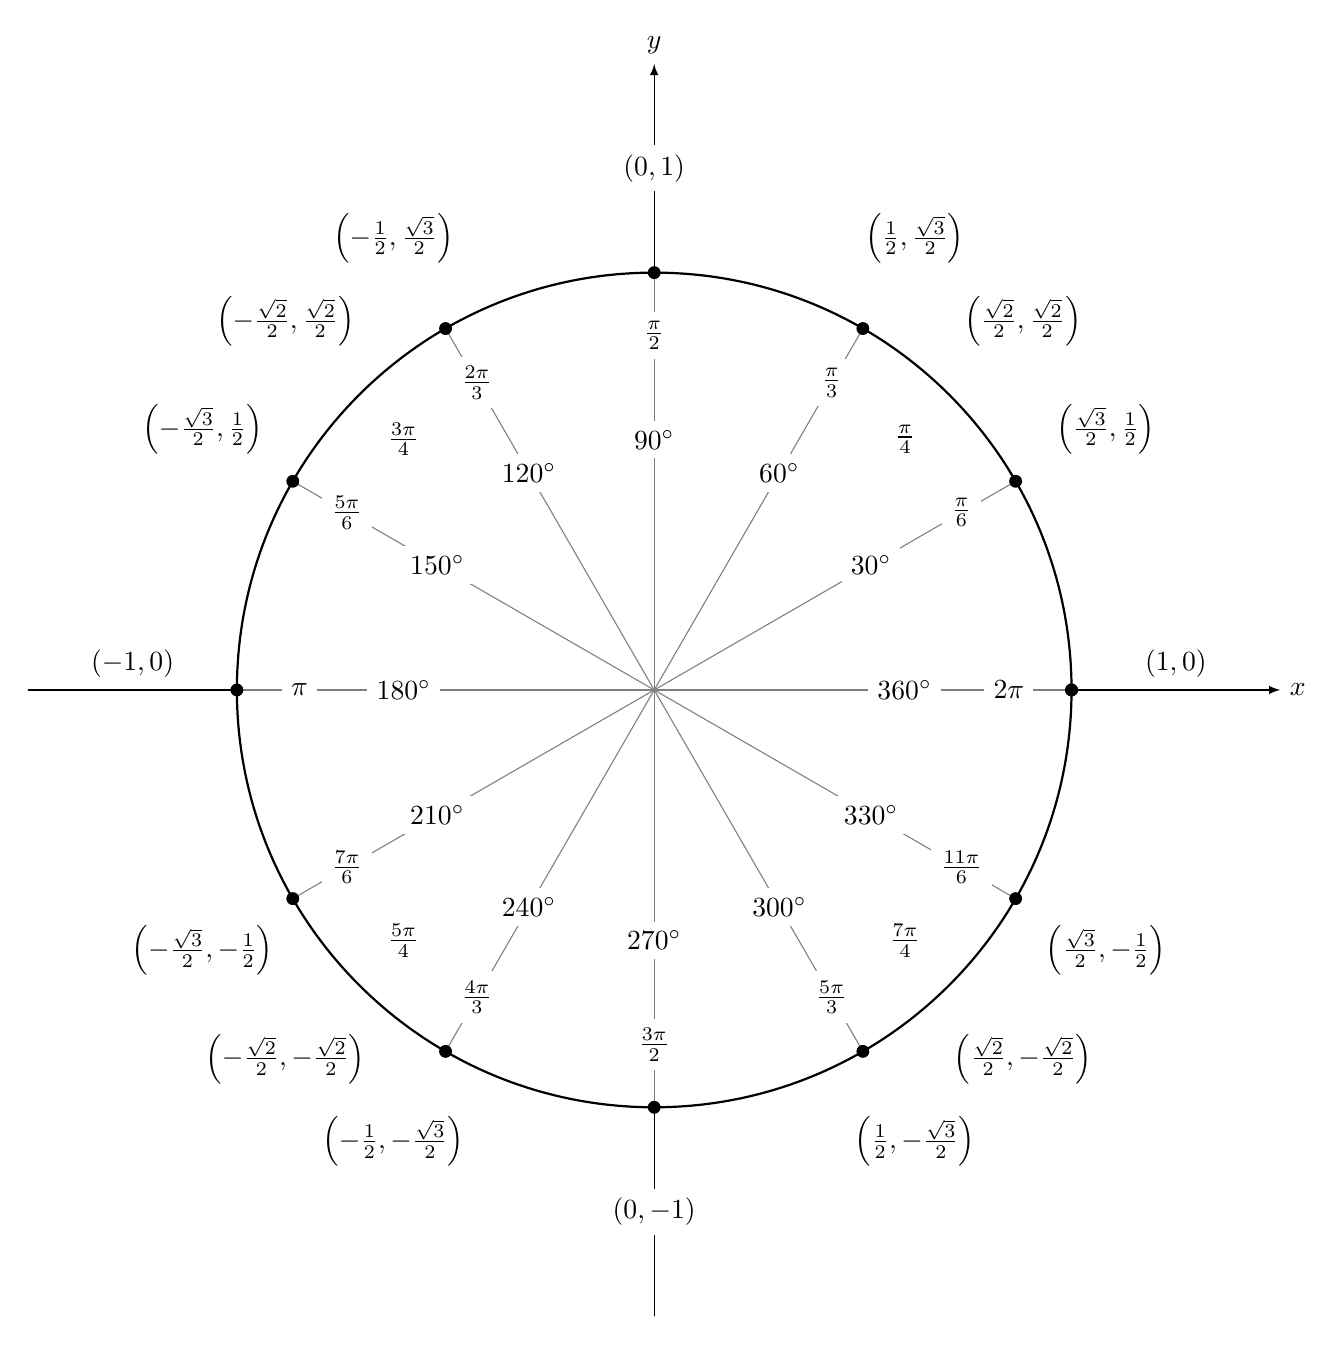
\begin{tikzpicture}[scale=5.3,cap=round,>=latex]
	% draw the coordinates
	\draw[->] (-1.5cm,0cm) -- (1.5cm,0cm) node[right,fill=white] {$x$};
	\draw[->] (0cm,-1.5cm) -- (0cm,1.5cm) node[above,fill=white] {$y$};

	% draw the unit circle
	\draw[thick] (0cm,0cm) circle(1cm);

	\foreach \x in {0,30,...,360} {
			% lines from center to point
			\draw[gray] (0cm,0cm) -- (\x:1cm);
			% dots at each point
			\filldraw[black] (\x:1cm) circle(0.4pt);
			% draw each angle in degrees
			\draw (\x:0.6cm) node[fill=white] {$\x^\circ$};
	}

	% draw each angle in radians
	\foreach \x/\xtext in {
		30/\frac{\pi}{6},
		45/\frac{\pi}{4},
		60/\frac{\pi}{3},
		90/\frac{\pi}{2},
		120/\frac{2\pi}{3},
		135/\frac{3\pi}{4},
		150/\frac{5\pi}{6},
		180/\pi,
		210/\frac{7\pi}{6},
		225/\frac{5\pi}{4},
		240/\frac{4\pi}{3},
		270/\frac{3\pi}{2},
		300/\frac{5\pi}{3},
		315/\frac{7\pi}{4},
		330/\frac{11\pi}{6},
		360/2\pi}
			\draw (\x:0.85cm) node[fill=white] {$\xtext$};

	\foreach \x/\xtext/\y in {
		% the coordinates for the first quadrant
		30/\frac{\sqrt{3}}{2}/\frac{1}{2},
		45/\frac{\sqrt{2}}{2}/\frac{\sqrt{2}}{2},
		60/\frac{1}{2}/\frac{\sqrt{3}}{2},
		% the coordinates for the second quadrant
		150/-\frac{\sqrt{3}}{2}/\frac{1}{2},
		135/-\frac{\sqrt{2}}{2}/\frac{\sqrt{2}}{2},
		120/-\frac{1}{2}/\frac{\sqrt{3}}{2},
		% the coordinates for the third quadrant
		210/-\frac{\sqrt{3}}{2}/-\frac{1}{2},
		225/-\frac{\sqrt{2}}{2}/-\frac{\sqrt{2}}{2},
		240/-\frac{1}{2}/-\frac{\sqrt{3}}{2},
		% the coordinates for the fourth quadrant
		330/\frac{\sqrt{3}}{2}/-\frac{1}{2},
		315/\frac{\sqrt{2}}{2}/-\frac{\sqrt{2}}{2},
		300/\frac{1}{2}/-\frac{\sqrt{3}}{2}}
			\draw (\x:1.25cm) node[fill=white] {$\left(\xtext,\y\right)$};

	% draw the horizontal and vertical coordinates
	% the placement is better this way
	\draw (-1.25cm,0cm) node[above=1pt] {$(-1,0)$}
		  (1.25cm,0cm)  node[above=1pt] {$(1,0)$}
		  (0cm,-1.25cm) node[fill=white] {$(0,-1)$}
		  (0cm,1.25cm)  node[fill=white] {$(0,1)$};
\end{tikzpicture}
\end{center}

\chapter{Review of Functions}
\section{Introduction}
This is the introduction section of my document.
\section{Linear Functions}
A linear function is a function that can be written in the form $f(x) = mx + b$, where $m$ is the slope of the line and $b$ is the $y$-intercept.

\subsection{Hyperbolic Functions}

Hyperbolic cosine 
\begin{equation}
	\cosh x = \frac{e^x + e^{-x}}{2}
\end{equation}



\chapter{Limits}
\section{Introduction}
This is the introduction section of my document.
\section{Intutive Definition of a Limit}

\begin{equation} 
    \lim_{x \to a} f(x) = L
\end{equation}

\begin{definition}
    {Definition of a Limit}
    The limit of a function $f(x)$ as $x$ approaches $a$ is $L$ if for every $\epsilon > 0$ there exists a $\delta > 0$ such that if $0 < |x - a| < \delta$, then $|f(x) - L| < \epsilon$.
\end{definition}

\begin{example}
    {Example 1}
  Enter an example here. 
\end{example}

\begin{important} 
    {Important} It is important that... 
\end{important}

\begin{formula}
    {Formula}
    Enter a formula here.
\end{formula}

\begin{proof}
    {Proof} This is a proof 
\end{proof}

\begin{equation} 
    s(t)= \text{position of the object at time $t$}
\end{equation}

\begin{example} 
{Example 2.2}
\[s(t)=16t^2+64\]
a) \([0.49, 0.50]\) \\
\begin{equation}
    \frac{s(0.5)-s(0.49)}{0.5-0.49}=-15.84
\end{equation}
b) \([0.50, 0.51]\) \\
\begin{equation}
    \frac{s(0.51)-s(0.5)}{0.51-0.5}=16.16u
\end{equation}

\end{example}



% Biblography 

\printbibliography

\end{document}